


\begin{minipage}{0.65\textwidth}

\begin{figure}[ht]
    \centering
    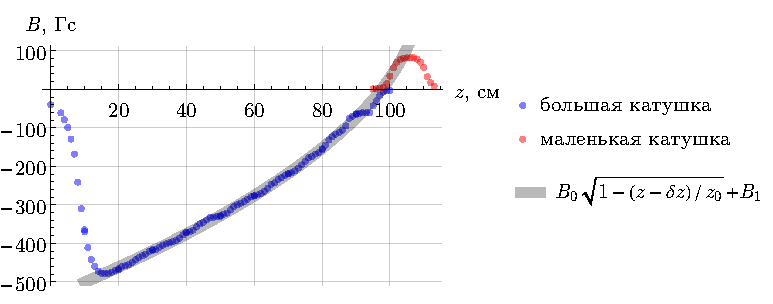
\includegraphics[width=0.9\textwidth]{../MOT/figs/Bz_v2.pdf}
    \caption{Зависимость магнитного поля внутри зеемановского замедлителя от координаты $z$. Ток маленькой катушки $\sub{I}{small} = 17\,$А, ток большой катушки $\sub{I}{big} = 35\,$А.}
\end{figure}


\end{minipage}
\hfill
\begin{minipage}{0.31\textwidth}

Тормозящая сила:
\begin{equation*}
    F = \frac{\hbar k \Gamma}{2} \frac{s}{1+s+4({\delta}+k v)^2/\Gamma^2}
\end{equation*}

\phantom{42}

Эффект Доплера:\\
\phantom{42} \hfill
$1\,\text{м}/\text{с} \sim 2\,\text{МГц}$

При этом: \\
\phantom{42} \hfill
$\Gamma \sim 10\,\text{МГц}$

Замедление \\
\phantom{4} 
от $150\,\text{м}/\text{с}$ до $\sub{v}{slow} \sim 30\,\text{м}/\text{с}$

\phantom{42}



Необходима подстройка резонанса магнитным полем:
\begin{equation*}
    \delta \to \delta + \mu B / \hbar
\end{equation*}


\end{minipage}